%!TEX root = ../vkr.tex

\section{Идеализированная атака}
\subsection{Извлечение сети глубины 0}
  Нейронная сеть глубины $0$ это линейная функция $ \mathnormal{f}( \mathnormal{x}) \equiv A^{\left (1\right)} \cdot  \mathnormal{x} + b^{\left(1\right)}$.
  Рассмотрим параллельные оценки $ \mathnormal{f}( \mathnormal{x})$ и $ \mathnormal{f}( \mathnormal{x}+\delta)$, причем $ \mathnormal{f}( \mathnormal{x}+\delta)- \mathnormal{f}( \mathnormal{x})=A^{\left (1\right)} \cdot \left( \mathnormal{x}+\delta\right)-A^{\left (1\right)} \cdot  \mathnormal{x} = A^{\left (1\right)} \cdot \delta$.
  Если $\delta = e_{i}$, $i$-ый стандартный базисный вектор из $\mathbb {R}^{d_{0}}$ $\left( \text{например, } e_{2}=\begin{bmatrix}0 & 1 & 0 & 0 & \dots & 0\end{bmatrix}\right)$, то $ \mathnormal{f}( \mathnormal{x}+\delta)- \mathnormal{f}( \mathnormal{x})= A^{\left (1\right)} \cdot \delta =  A_{i}^{\left (1\right)}$.
  Это позволяет непосредственно считать веса $A_{i}^{\left (1\right)}$. Т.е. мы находим конечные разности для оценки градиента $ \mathnormal{f}$, заданного ${\nabla}_{ \mathnormal{x}} \mathnormal{f}( \mathnormal{x}) \equiv A_{i}^{\left (1\right)}$.
 \begin{figure}[h]
\center{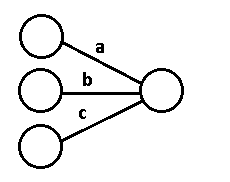
\includegraphics[width=0.25\linewidth]{0-deep}}
\end{figure}


\subsection{Извлечение сети глубины 1}
\Def {Функция, вычисляющая первые первые $j$ слоёв $ \mathnormal{f}$ $\left ( \text{до }  \mathnormal{f}_{j} \text{ включительно, но не включая } \sigma \right )$, обозначается как  $ \mathnormal{f}_{1..j}$. В частности, $ \mathnormal{f}= \mathnormal{f}_{1..k}$.}
\Def {$\mathcal{V} \left ( \eta {;}  \mathnormal{x} \right )$ обозначает вход нейрона $\eta$ $\left ( \text{до применения } \sigma \right)$ при оценке в $\mathnormal{x}$. $\mathcal{L}(\eta)$ обозначает слой нейрона $\eta$. Первый слой начинается с 1.}
\Def { Нейрон $\eta$ находится в критической точке, когда $\mathcal{V} \left ( \eta {;}  \mathnormal{x} \right ) = $ 0. Свидетелем того, что $\eta$ находится в критической точке, назовём входной сигнал $\mathnormal{x}$, обозначаемый $\mathnormal{x} \in \mathcal{W}(\eta)$. Если $\mathcal{V} \left ( \eta {;}  \mathnormal{x} \right ) > $ 0 тогда нейрон активен, иначе $-$ неактивен.}

 \begin{figure}[h]
\center{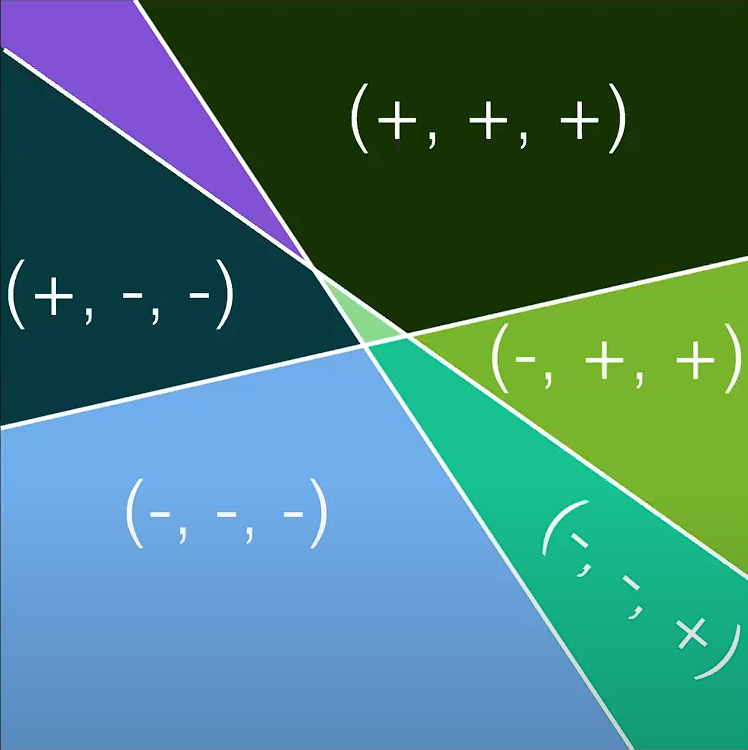
\includegraphics[width=0.6\linewidth]{1-deep}}
\caption{Разбиение входного пространства нейронами 1-го слоя}
\label{ris:1-deep}
\end{figure}

\subsection {Извлечение строк $A^{\left(1\right)}$ с точностью до знака}
\begin{itemize}
\item
  Предположим, что нам дан свидетель $\mathnormal{x}^{*} \in {\mathcal{W}}(\eta_{j})$ для которого нейрон $\eta_{j}$ будет находиться в критической точке. Далее предположим, что только $\eta_{j}$ находится в критической точке, а для остальных нейоронов $\eta \neq \eta_{j}$ имеем $\left |\mathcal{V} \left ( \eta {;}  \mathnormal{x_{j}} \right ) \right | > \delta > 0$.
\item
  $e_{i}$ $-$ стандартные базисные вектора в ${\mathcal{X}}=\mathbb{R}^{N}$. Запросами по двум парам входов $\left({\mathnormal{x}^{*}}, {\mathnormal{x}^{*}}+\epsilon e_{i}\right)$ и  $\left({\mathnormal{x}^{*}}, {\mathnormal{x}^{*}}-\epsilon e_{i}\right)$ мы можем оценить
$\alpha_{+}^{i}=\left . \frac{\partial \mathnormal{f(x)}}{\partial e_{i}} \right|_{\mathnormal{x}=\mathnormal{x}^{*}+\epsilon e_{i}}$ и $\alpha_{-}^{i}=\left . \frac{\partial \mathnormal{f(x)}}{\partial e_{i}}\right|_{\mathnormal{x}=\mathnormal{x}^{*}-\epsilon e_{i}}$ с помощью конечных разностей.
\item
  Рассмотрим величину $\left | \alpha_+ - \alpha_- \right |$. Если никакие два столбца в $A^{\left(1\right)}$ не коллинеарны и пока $\epsilon < \frac{\delta}{\sum_{i,j}\left|A_{i,j}^{\left(1\right)}\right|}$, мы гарантируем, что все нейроны $\eta \neq \eta_{j}$ остаются в одном и том же состоянии.
  \end{itemize}
